\documentclass[onecolumn]{article}
\usepackage[a4paper]{geometry}
\usepackage[hyphens]{url}
\usepackage{datetime}
\usepackage[margin=2em, font=small,labelfont=it]{caption}
\usepackage{graphicx}
\usepackage{mathpazo} % use palatino
\usepackage[scaled]{helvet} % helvetica
\usepackage{microtype}
\usepackage{amsmath}
\usepackage{booktabs}
% Letterspacing macros
\newcommand{\spacecaps}[1]{\textls[200]{\MakeUppercase{#1}}}
\newcommand{\spacesc}[1]{\textls[50]{\textsc{\MakeLowercase{#1}}}}
\usepackage[utf8]{inputenc}
\usepackage[T1]{fontenc}
\usepackage{hyperref}
\hypersetup{
    colorlinks=true,
    linkcolor=blue,
    filecolor=magenta,
    urlcolor=cyan,
}

\begin{document}

\title{\spacecaps{End-to-End Encrypted Chat System with Metadata-Based Anomaly Detection}\\ \normalsize \spacesc{CENG3544: Computer Network and Security} }

\author{Hakan Kayac\i\\hakankayaci@posta.mu.edu.tr\\[6pt]Instructor: Do\c{c}.\ Dr.\ Enis Karaarslan}
\date{\today}

\maketitle

\begin{abstract}
Chat messages usually pass through a central server that can read everything it forwards. This project is a small terminal-based chat application that makes this problem visible and shows two defences against it. Two clients talk through a central TCP relay. In plain mode the server prints the messages, so anyone watching it can read them. In encrypted mode the clients agree on a key with X25519 and encrypt with AES-256-GCM, so the server sees only ciphertext; a single flipped bit is rejected by the receiver, which demonstrates message integrity. A local security agent looks only at connection metadata --- never at the message body --- and uses simple rules plus an Isolation Forest to flag a safe, simulated attacker. Everything runs on one machine and performs no real attacks.
\end{abstract}

\section{Introduction}

In almost every chat application the two users do not talk directly; their messages go through a server in the middle that forwards traffic. That server is a single point where all messages are visible, so whoever controls it --- or breaks into it --- can read them. The usual fix is end-to-end encryption: the two endpoints share a secret the server never learns, the sender encrypts before the message leaves, and only the receiver can decrypt. What a teaching project rarely shows is the difference in action: the same server reading a message in one mode and failing to read it in another.

A second problem is that the operator still wants to keep the service healthy --- stop flooding, notice reconnection storms, react to tampering --- but reading the messages to do so would defeat the encryption. So we also ask how much can be detected from metadata alone. This project brings both ideas together in one small system. Its contributions are: a chat application with a plain and an encrypted mode and a server ``spy view'' that shows exactly what a relay can read; an encrypted mode built on X25519 and AES-256-GCM with a live tamper-detection demo; and a metadata-only security agent (rules plus an Isolation Forest) with a safe, localhost-only attacker simulator.\footnote{Source code: \url{https://github.com/hakankayaci/computer-network-security-final}} Section~\ref{sec:fundamentals} reviews the concepts, Section~\ref{sec:related} the related work, Section~\ref{sec:proposal} the system, Section~\ref{sec:implementation} the implementation, Section~\ref{sec:results} the results, and Section~\ref{sec:conclusion} the conclusion.

\section{Fundamentals}
\label{sec:fundamentals}

\textbf{Key agreement.} Two parties can agree on a shared secret over a public channel, which is the Diffie--Hellman idea~\cite{c1}. We use X25519~\cite{c2,c3}, the elliptic-curve version used by TLS~1.3 and Signal, and pass its output through HKDF~\cite{c4} to get a clean 256-bit key. Each side computes the key locally, so a relay that only forwards the public keys cannot reconstruct it.

\textbf{Authenticated encryption.} AES in Galois/Counter Mode~\cite{c5,c6} encrypts and authenticates at the same time: it adds a tag over the message, and if any ciphertext bit changes, the receiver's check fails and the message is refused. This gives confidentiality and integrity in one step~\cite{c7}.

\textbf{Anomaly detection.} Instead of matching known signatures, anomaly detection learns what normal looks like and flags outliers~\cite{c8}. The Isolation Forest~\cite{c9} does this without labels and works on small tabular inputs, so it can score metadata such as message rate and reconnection count. We use the scikit-learn implementation~\cite{c15}. We assume an honest-but-curious server and a misbehaving client; protecting the key exchange against an active man-in-the-middle is out of scope.

\section{Related Works}
\label{sec:related}

Production messengers built on the Signal protocol give strong end-to-end guarantees and are the model we take inspiration from; secure messaging as a whole has been surveyed in~\cite{c8b}. TLS~1.3~\cite{c10} protects data in transit, but a server that terminates TLS still sees the plaintext, whereas our encrypted mode keeps the relay blind. On the detection side, machine learning is widely used for intrusion detection~\cite{c12}, and Sommer and Paxson~\cite{c13} explain why false positives make it hard in practice. Most such systems read packet contents; the difference here is that our detector is restricted to metadata, so detection and confidentiality can coexist. Table~\ref{tab:compare} summarises the comparison.

\begin{table}[htbp]
\centering
\caption{Where the project sits relative to related approaches.}
\label{tab:compare}
\small
\begin{tabular}{@{}lcccc@{}}
\toprule
 & \textbf{End-to-end} & \textbf{Relay sees} & \textbf{Built-in abuse} & \textbf{Detection on} \\
\textbf{Approach} & \textbf{encryption} & \textbf{content} & \textbf{detection} & \textbf{metadata only} \\
\midrule
TLS (transport)       & No (hop-by-hop) & Yes           & No      & --- \\
Signal / WhatsApp     & Yes             & No            & Partial & Partial \\
Typical ML-based IDS  & ---             & Yes (payload) & Yes     & No \\
\textbf{This project} & Yes             & No            & Yes     & Yes \\
\bottomrule
\end{tabular}
\end{table}

\section{System Proposal}
\label{sec:proposal}

The system is a central relay with clients around it (Figure~\ref{fig:arch}). Two clients connect to a central TCP server and exchange messages through it; the server only forwards them and observes what it forwards, while also logging metadata and running a security agent. In plain mode the clients send text without protection and the spy view prints it in full. In encrypted mode the clients first run an X25519 exchange (relayed by the server) and then encrypt with AES-256-GCM, so the spy view shows only ciphertext. Both modes share the same relay code, which makes the contrast easy to show.

\begin{figure}[htbp]
\centering
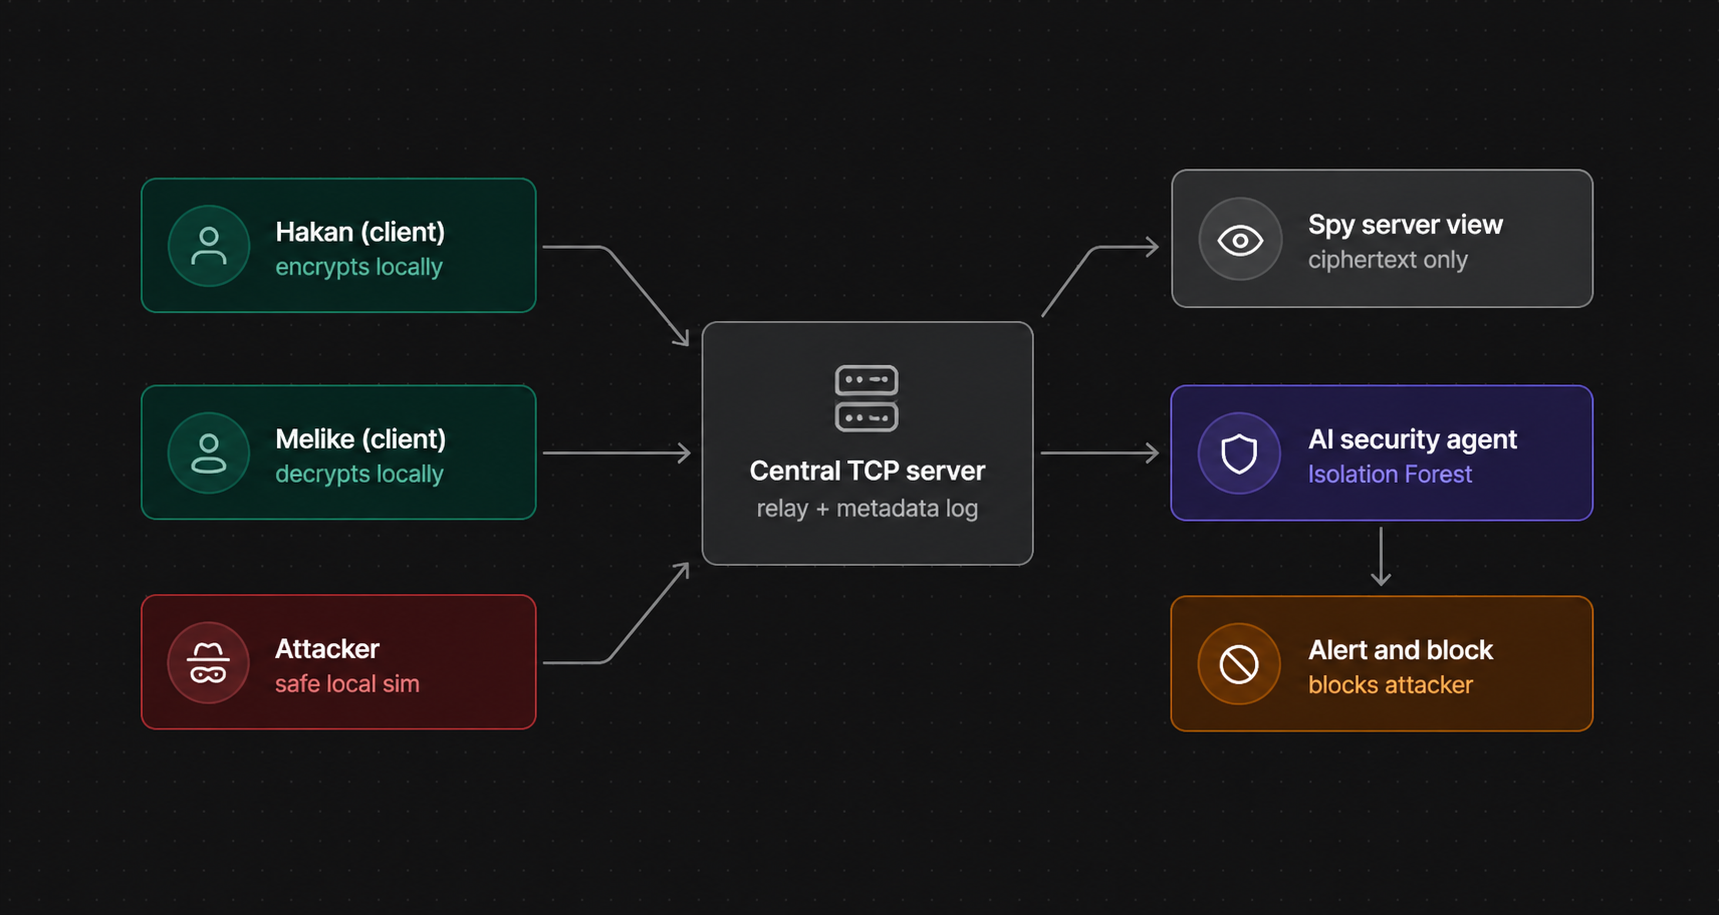
\includegraphics[width=0.9\linewidth]{images/1.png}
\caption{System architecture. Clients encrypt and decrypt locally; the server relays ciphertext and logs metadata; the security agent reads only metadata and can alert and block the safe attacker simulation.}
\label{fig:arch}
\end{figure}

A message passes through five stages (Figure~\ref{fig:flow}): key setup, encryption, relay with the spy view, integrity verification at the receiver, and a metadata-based response. The first four protect every message; the fifth runs continuously over the metadata. Three principles guided the design: everything stays local and safe (loopback only, no real attacks); the detector is privacy-preserving by construction (metadata only); and detection is explainable first, with rules as the primary decision and the Isolation Forest as a secondary signal.

\begin{figure}[htbp]
\centering
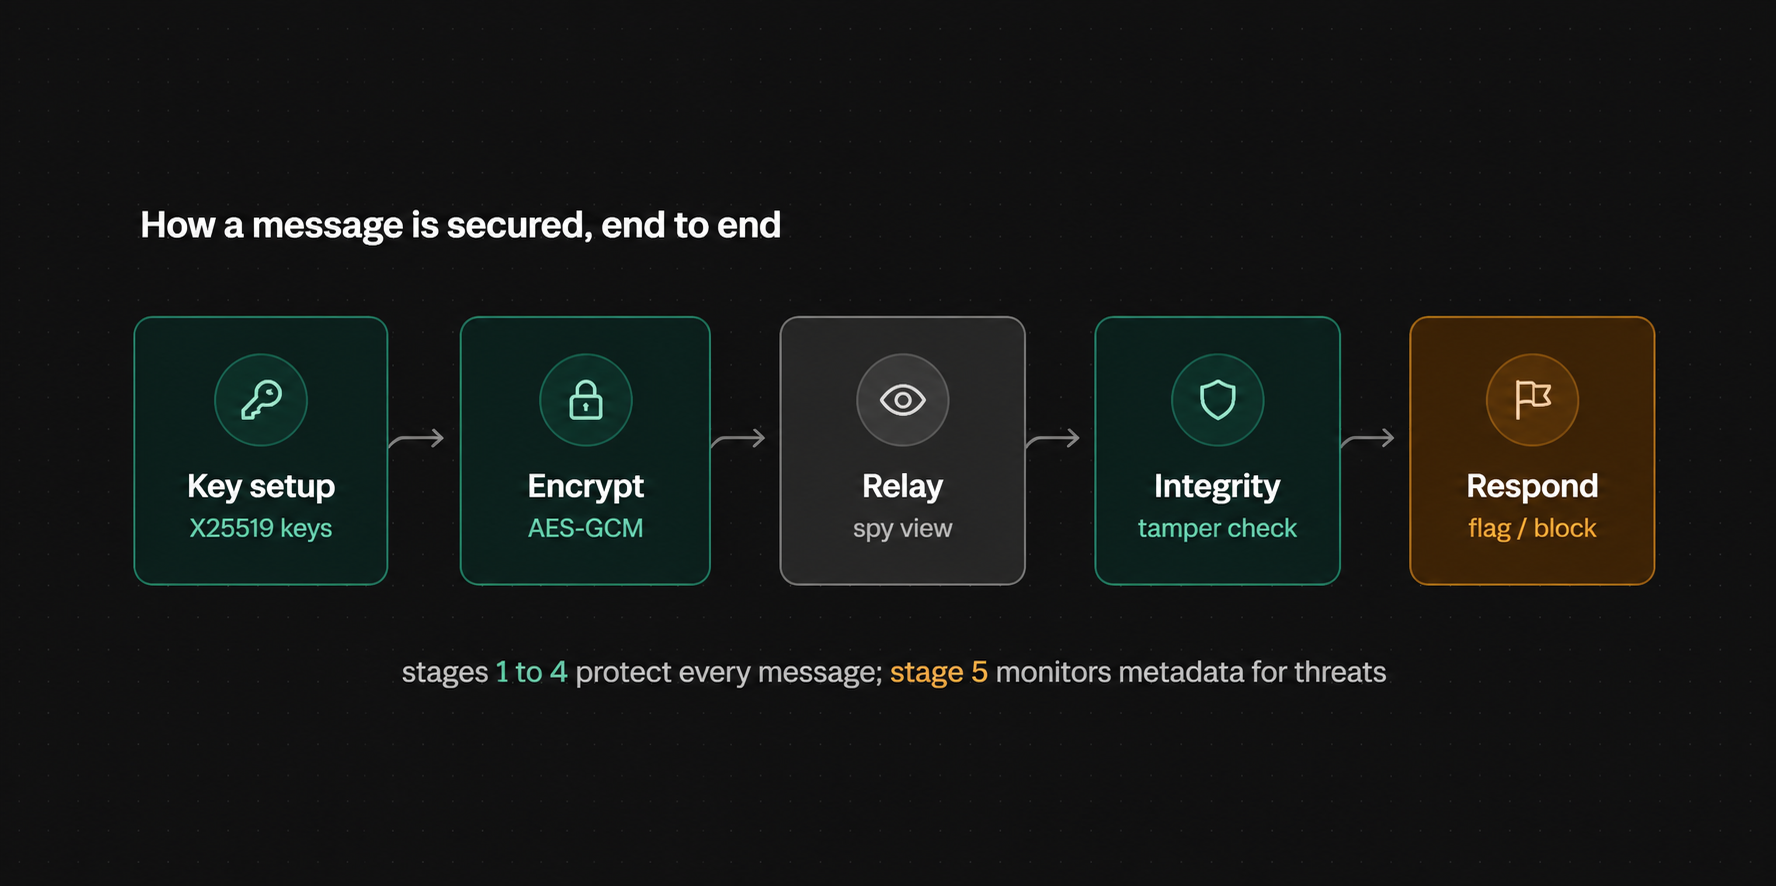
\includegraphics[width=0.9\linewidth]{images/2.png}
\caption{The five-stage security flow of a message: key setup, encryption, relay, integrity verification, and metadata-based response.}
\label{fig:flow}
\end{figure}

\section{Implementation}
\label{sec:implementation}

The prototype is written in Python~3.8 with only free, open-source libraries and needs no special hardware. Networking uses the standard \texttt{socket} module with one thread per client plus a background thread for the agent; cryptography uses the \texttt{cryptography} library (X25519, AES-GCM, HKDF-SHA256) and detection uses \texttt{scikit-learn}. Clients and server exchange one JSON object per line, with message types for registration, public-key relay, chat, integrity reports, and the safe tamper request. For an encrypted message the sender uses a fresh 12-byte nonce and AES-256-GCM; the receiver decrypts locally and refuses the message if the tag does not match.

The agent never reads message bodies. Per client, it computes a short feature vector from the metadata log --- messages per minute, average size, reconnection count, tampering-attempt count, average interval, burst count, and connection-attempt count --- and scores it with weighted rules and the Isolation Forest, taking the stronger score. Two decisions came out of testing: the model is not allowed to raise an alert on its own for a quiet client, which stopped ordinary users from being flagged; and a tampering event is attributed to the attacker who caused it, not to the victim who reports the failed check, which fixed a case where the victim was being blocked. The attacker simulator (\texttt{attacker\_simulation.py}) connects only to the local server and produces suspicious patterns --- a tamper request, repeated reconnections, spam, and an oversized message --- and ends cleanly when the agent blocks it. We evaluated four scenarios: plaintext visibility in plain mode, ciphertext-only relay in encrypted mode, tamper detection, and attacker detection.

\section{Results and Discussion}
\label{sec:results}

In plain mode the spy view printed the full message, confirming that the relay reads everything when no protection is used. In encrypted mode the same view printed only a ciphertext preview while the receiver showed the decrypted text, which is the central result: the relay still forwards messages but can no longer read them. Flipping one bit of a ciphertext made the receiver's AES-GCM check fail, so the message was refused and an integrity warning was shown.

For detection, the attacker was reliably marked suspicious (risk around 0.83) with a reason listing the tampering attempt, repeated reconnections, burst traffic, and the model's anomaly, and was then temporarily blocked; the two ordinary users were never flagged while chatting normally, even right after a victim reported a tampered message. Reaching that last outcome needed the two fixes above, and it is a small concrete example of the false-positive problem that the literature warns about~\cite{c13}: a detector that punishes the wrong party is worse than none. The overhead is negligible and the whole system runs on one ordinary machine.

\section{Conclusion}
\label{sec:conclusion}

We built a small chat system that makes a familiar problem tangible and then defends against it. In plain mode the server reads every message; in encrypted mode the clients agree on a key with X25519 and encrypt with AES-256-GCM, so the server sees only ciphertext and tampering is caught at the receiver. A separate agent watches metadata, never the message body, and flags and blocks a simulated attacker while leaving ordinary users alone.

The design has clear limits. Public keys are relayed without authentication, so a malicious server could mount a man-in-the-middle attack; there is no replay protection, no real user authentication, and the model is trained on a synthetic baseline, while the block is name-based and easy to evade. These are also the next steps: authenticated key exchange with key fingerprints, sequence numbers against replay, training on real traffic, more metadata features, and automated tests.

\section*{Acknowledgement}

We thank our course instructor, Do\c{c}.\ Dr.\ Enis Karaarslan, for guidance throughout the project and for feedback on the design and the report.

\begin{thebibliography}{00}
\bibitem{c1} W. Diffie and M. E. Hellman, ``New directions in cryptography,'' \emph{IEEE Transactions on Information Theory}, vol.~22, no.~6, pp.~644--654, 1976.
\bibitem{c2} D. J. Bernstein, ``Curve25519: New Diffie--Hellman speed records,'' in \emph{Public Key Cryptography (PKC)}, Springer, 2006, pp.~207--228.
\bibitem{c3} A. Langley, M. Hamburg, and S. Turner, ``Elliptic Curves for Security,'' RFC~7748, IETF, 2016.
\bibitem{c4} H. Krawczyk and P. Eronen, ``HMAC-based Extract-and-Expand Key Derivation Function (HKDF),'' RFC~5869, IETF, 2010.
\bibitem{c5} D. McGrew and J. Viega, ``The Galois/Counter Mode of Operation (GCM),'' Submission to NIST, 2004.
\bibitem{c6} M. Dworkin, ``Recommendation for Block Cipher Modes of Operation: Galois/Counter Mode (GCM) and GMAC,'' NIST Special Publication 800-38D, 2007.
\bibitem{c7} M. Bellare and C. Namprempre, ``Authenticated encryption: Relations among notions and analysis of the generic composition paradigm,'' in \emph{ASIACRYPT}, Springer, 2000, pp.~531--545.
\bibitem{c8} V. Chandola, A. Banerjee, and V. Kumar, ``Anomaly detection: A survey,'' \emph{ACM Computing Surveys}, vol.~41, no.~3, pp.~1--58, 2009.
\bibitem{c8b} N. Unger, S. Dechand, J. Bonneau, S. Fahl, H. Perl, I. Goldberg, and M. Smith, ``SoK: Secure messaging,'' in \emph{IEEE Symposium on Security and Privacy}, 2015, pp.~232--249.
\bibitem{c9} F. T. Liu, K. M. Ting, and Z.-H. Zhou, ``Isolation forest,'' in \emph{IEEE International Conference on Data Mining (ICDM)}, 2008, pp.~413--422.
\bibitem{c10} E. Rescorla, ``The Transport Layer Security (TLS) Protocol Version 1.3,'' RFC~8446, IETF, 2018.
\bibitem{c12} A. L. Buczak and E. Guven, ``A survey of data mining and machine learning methods for cyber security intrusion detection,'' \emph{IEEE Communications Surveys \& Tutorials}, vol.~18, no.~2, pp.~1153--1176, 2016.
\bibitem{c13} R. Sommer and V. Paxson, ``Outside the closed world: On using machine learning for network intrusion detection,'' in \emph{IEEE Symposium on Security and Privacy}, 2010, pp.~305--316.
\bibitem{c14} P. Garcia-Teodoro, J. Diaz-Verdejo, G. Macia-Fernandez, and E. Vazquez, ``Anomaly-based network intrusion detection: Techniques, systems and challenges,'' \emph{Computers \& Security}, vol.~28, no.~1--2, pp.~18--28, 2009.
\bibitem{c15} F. Pedregosa et al., ``Scikit-learn: Machine learning in Python,'' \emph{Journal of Machine Learning Research}, vol.~12, pp.~2825--2830, 2011.
\end{thebibliography}
\vspace{12pt}

\end{document}
